%%%%%%%%%%%%%%%%%%%%%%%%%%%%%%%%%%%%%%%%%
% a0poster Landscape Poster
% LaTeX Template
% Version 1.0 (22/06/13)
%
% The a0poster class was created by:
% Gerlinde Kettl and Matthias Weiser (tex@kettl.de)
% 
% This template has been downloaded from:
% http://www.LaTeXTemplates.com
%
% License:
% CC BY-NC-SA 3.0 (http://creativecommons.org/licenses/by-nc-sa/3.0/)
%
%%%%%%%%%%%%%%%%%%%%%%%%%%%%%%%%%%%%%%%%%

%----------------------------------------------------------------------------------------
%	PACKAGES AND OTHER DOCUMENT CONFIGURATIONS
%----------------------------------------------------------------------------------------

\documentclass[a0b,landscape]{a0poster}

\usepackage{multicol} % This is so we can have multiple columns of text side-by-side
\columnsep=100pt % This is the amount of white space between the columns in the poster
\columnseprule=3pt % This is the thickness of the black line between the columns in the poster

\usepackage[svgnames]{xcolor} % Specify colors by their 'svgnames', for a full list of all colors available see here: http://www.latextemplates.com/svgnames-colors

\usepackage{times} % Use the times font
%\usepackage{palatino} % Uncomment to use the Palatino font

\usepackage{graphicx} % Required for including images
\graphicspath{{figures/}} % Location of the graphics files
\usepackage{booktabs} % Top and bottom rules for table
\usepackage[font=small,labelfont=bf]{caption} % Required for specifying captions to tables and figures
\usepackage{amsfonts, amsmath, amsthm, amssymb} % For math fonts, symbols and environments
\usepackage{wrapfig} % Allows wrapping text around tables and figures
\usepackage{mathtools}
\newcommand{\pl}{\partial}
\DeclarePairedDelimiter{\bigP}{\big(}{\big)}
\DeclarePairedDelimiter{\BigP}{\Big(}{\Big)}
\DeclarePairedDelimiter{\biggP}{\bigg(}{\bigg)}
\DeclarePairedDelimiter{\BiggP}{\Bigg(}{\Bigg)}
\DeclarePairedDelimiter{\bigBk}{\big[}{\big]}
\DeclarePairedDelimiter{\BigBk}{\Big[}{\Big]}
\DeclarePairedDelimiter{\biggBk}{\bigg[}{\bigg]}
\DeclarePairedDelimiter{\BiggBk}{\Bigg[}{\Bigg]}
\DeclarePairedDelimiter{\bigBc}{\big\{}{\big\}}
\DeclarePairedDelimiter{\BigBc}{\Big\{}{\Big\}}
\DeclarePairedDelimiter{\biggBc}{\bigg\{}{\bigg\}}
\DeclarePairedDelimiter{\BiggBc}{\Bigg\{}{\Bigg\}}
\newcommand{\lcm}{\text{lcm}}
\newcommand{\Leib}[3]{\frac{\partial^{#1} #2}{\partial #3^{#1}}}
\newcommand{\atan}{\text{atan}}
\newcommand{\diff}[2]{\frac{d#1}{d#2}}
\newcommand{\pdif}[2]{\frac{\pl #1}{\pl #2}}
\begin{document}

%----------------------------------------------------------------------------------------
%	POSTER HEADER 
%----------------------------------------------------------------------------------------

% The header is divided into three boxes:
% The first is 55% wide and houses the title, subtitle, names and university/organization
% The second is 25% wide and houses contact information
% The third is 19% wide and houses a logo for your university/organization or a photo of you
% The widths of these boxes can be easily edited to accommodate your content as you see fit

\begin{minipage}[b]{0.80\linewidth}
\veryHuge \color{Red} \textbf{Applications of Imaginary Time Propagation Method in Material Research} \color{Black}\\ % Title
\huge \textbf{Frisly Gonzalez, Joshua Cook, and Jussi Eloranta}\\ % Author(s)
\huge California State University, Northridge\\ Department of Chemistry and Biochemistry
\end{minipage}
%
%
\begin{minipage}[b]{0.19\linewidth}

\includegraphics[width=10cm]{CSUNSeal.pdf} % Logo or a photo of you, adjust its dimensions here
\end{minipage}

\vspace{1cm} % A bit of extra whitespace between the header and poster content

%----------------------------------------------------------------------------------------

\begin{multicols}{3} % This is how many columns your poster will be broken into, a poster with many figures may benefit from less columns whereas a text-heavy poster benefits from more


%----------------------------------------------------------------------------------------
%	INTRODUCTION - MATHEMATICAL  %----------------------------------------------------------------------------------------

\color{Black} % SaddleBrown color for the introduction

\section*{the Imaginary Time Propagation}

The imaginary time propagation method (ITP) relies on solving the
time-dependent Schrödinger equation in imaginary time. We perform a Wick Rotation (setting \(t=-i\tau\)) to transform the time-dependent Schrödinger into a simple diffusion equation

\begin{equation}
\label{eq:itpSch}
\frac{\partial \psi(r,\tau)}{\partial
\tau}=-\frac{\hat{H}}{\hbar}\psi(r,\tau) \implies \psi(r,\tau)=\exp(-\hat{H}\tau/\hbar)\psi(r,0)
\end{equation}

\paragraph{Iterative Solutions to Eigenproblems}This can be thought of as the analog to a power solution or subspace iteration. As \(\tau\to\infty\), \(\psi(r,\tau)\) will converge on the eigenfunction for the ground state.

% In practice, a random vector is chosen as the initial state. A time-propagation will yield the ground state eigenvector. If a vector other than the ground state is desired, \(N\) separate wave functions are propagated. Each higher state eigenvector is required to be orthogonal to the lower eigenvectors and are thus discovered through the iterative process. Approximate orthogonality is enforced in the following way.

%\begin{equation}
%\label{eq:appxOrth}
%\pdif{\psi_i(r,\tau)}{\tau} = -\frac{\hat{H}}{\hbar}\psi(r,\tau)-\lambda\sum_{j < i}^N %|\langle \psi_j(r,\tau)|\psi_i(r,\tau)\rangle|^2
%\end{equation}

\paragraph{} In order to implement the solution computationally, the exponential
operator is approximated using the Cayley unitary form, transforming the eigenvalue problem into a linear problem:

\begin{equation}
\label{eq:CayleyExpansion}
\exp(-H\Delta\tau)\approx\biggP{1+\frac{1}{2}H\Delta\tau}^{-1}\biggP{1-\frac{1}{2}H\Delta\tau} \implies \biggP{1+\frac{1}{2}H\Delta\tau}\psi(r,\tau+\Delta\tau)=\biggP{1-\frac{1}{2}H\Delta\tau}\psi(r,\tau)
\end{equation}

\paragraph{Stopping Criteria}
A formula for the absolute error, \(\Delta E_i\) present in \(E_i(\tau)\) can be written in terms of the quantum mechanical standard deviation of \(H\) and is used as a stopping criteria.

\begin{equation}
\label{eq:error}
\Delta E_i = |E_i -\langle\psi_i(r,\tau)|H|\psi_i(r,\tau)|\leq\sqrt{2}\sqrt{\langle\psi_i(r,\tau)|H^2|\psi_i(r,\tau)\rangle-\langle\psi_i(r,\tau)|H|\psi_i(r,\tau)\rangle^2}
\end{equation}

%----------------------------------------------------------------------------------------
%	Mathematical Methods
%----------------------------------------------------------------------------------------

\color{Black} % Navy color for the abstract

\section*{Applications to Bosonic Density Functional Theory}

Helium clusters were modeled by the Orsay-Trento DFT (OT-DFT) and the
interaction with the guest molecule was included through an external
potential. To compute the effective moment of inertia of the
molecule--helium complex, we include an additional energy term of the
form \(-\omega L_z\) and compute the ``rotating'' groundstate energy by
minimizing

\begin{equation}
\label{eq:OTDFT}
E[\Psi,\omega]=\int\biggBc{\frac{\hbar^2}{2m}|\nabla\Psi|^2+\epsilon_{OT}[\Psi]+V_{X-\text{He}}|\Psi|^2-\omega \Psi*L_z\Psi}
\end{equation}

The non-linear Schrödinger-type equation arising from the minimization
of eq. 4 is solved by means of imaginary time propagation.

%----------------------------------------------------------------------------------------
%	RESULTS - MATHEMATICAL
%----------------------------------------------------------------------------------------

 
\section*{Results}
The ITP method reduces the solving of an eigenproblem to an iterative power solution via the solution of a linear equation. 
% ITP is being implemented in practice parallelized, using C and openBLAS. 
In current practice has been shown to have better scalability than the implicitly restarted Lanczos method as implemented in ARPACK. 

For the purposes of training, the algorithm is being reimplemented in Python and Numpy/Scipy. The solution of the linear equation being the most computationally expensive, theoretically involving a matrix inversion at each iteration, seven linear solution schemes were speed-tested versus Numpy's built-in eigensolver: the Numpy solver, the Scipy solver, Scipy's conjugate gradient squared (CGS) solver, a Cholevsky decomposition method, two of Scipy's sparse solvers, and a pre-inversion of the matrix iterated. 
\begin{center}\vspace{1cm}
\minipage{0.10\textwidth}
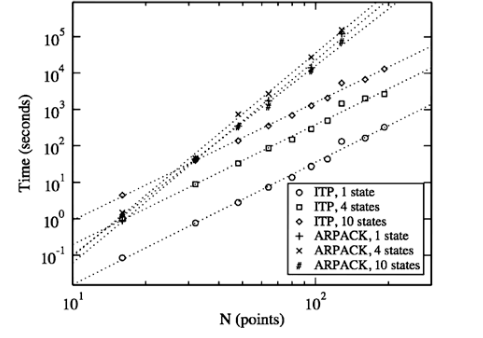
\includegraphics[width=\linewidth]{itpvlanc.png}
\captionof{figure}{\color{Navy} Computational scaling of the ITP and implicitly restarted Lanczos methods (ARPACK) for 1, 4 and 10 states.}
\endminipage\hfill
\minipage{0.10\textwidth}
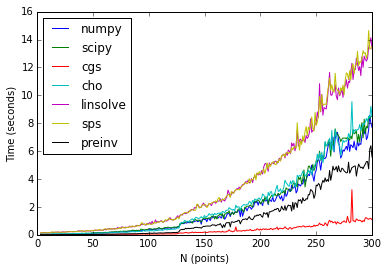
\includegraphics[width=\linewidth]{analysis_9_1.png}
\captionof{figure}{\color{Navy} Implementation of seven linear solving schemes in Python.}
\endminipage\hfill
\minipage{0.10\textwidth}
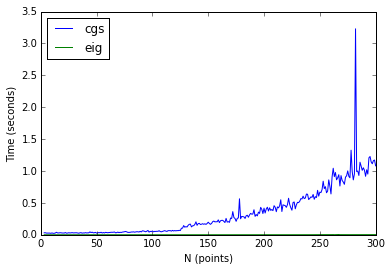
\includegraphics[width=\linewidth]{analysis_10_1.png}
\captionof{figure}{\color{Navy} Conjugate Gradient Squared Solver ITP v Built-in Eigensolver}
\endminipage
\end{center}\vspace{1cm}

The CGS solver was found to be the fastest. In comparison to the built-in eigensolver, however, it falls well short of reasonable performance standards. Furthermore, the CGS method has been found to be the least stable of the methods (note the spike at $N\approx 280$).

\columnbreak

%----------------------------------------------------------------------------------------
%	ABSTRACT
%----------------------------------------------------------------------------------------

\color{Navy} % Navy color for the abstract

\begin{abstract}

Helium droplets not only provide a unique matrix environment for high resolution spec- troscopy and studying molecular solvation but also allow to use guest molecules as probes of the surrounding quantum medium.1–3 After the initial discovery of the helium droplet tech- nique for spectroscopic applications, attention quickly turned into characterizing the physical properties of the helium droplets themselves. The groundbreaking experiments by the Toen- nies group employed the glyoxal molecule as a probe to study the helium droplet response through optical absorption spectrum.
\end{abstract}

%----------------------------------------------------------------------------------------
%	RESULTS 
%----------------------------------------------------------------------------------------
\color{Black}

\section*{Bosonic Density Functional Theory}
In the experiment, bosonic density functional theory (DFT) is the method used to obtain calculated rotational constant values.  Density functional theory is a technique that plays an important role in determining the key components that can explain why the moment of inertia decreases when rotational superfluidity takes place. The results obtained using DFT are compared with experimental data and Quantum Monte Carlo (QMC) values and there is a similar agreement which is shown by the appearance firs-turn over point.  

The first minimum appearing in molecular rotational constants as a function of helium droplet size has been previously associated with the onset of superfluidity in these finite systems. We investigate this relationship by bosonic density functional theory calculations of classical molecular rotors (OCS, N2O, CO and HCN) interacting with the surrounding helium. The calculated rotational constants are in fair agreement with the existing experimental data, demonstrating the applicability of the theoretical model. By inspecting the spatial evolution of the global phase and density, the increase in the rotational constant after the first minimum is shown to correlate with continuous coverage of the molecule by helium and appearance of angular phase coherence rather than completion of the first solvent shell. We assign the observed phenomenon to quantum phase transition between a localized state and one-dimensional superfluid, which represents the onset of rotational superfluidity in small helium droplets.

\begin{center}\vspace{1cm}
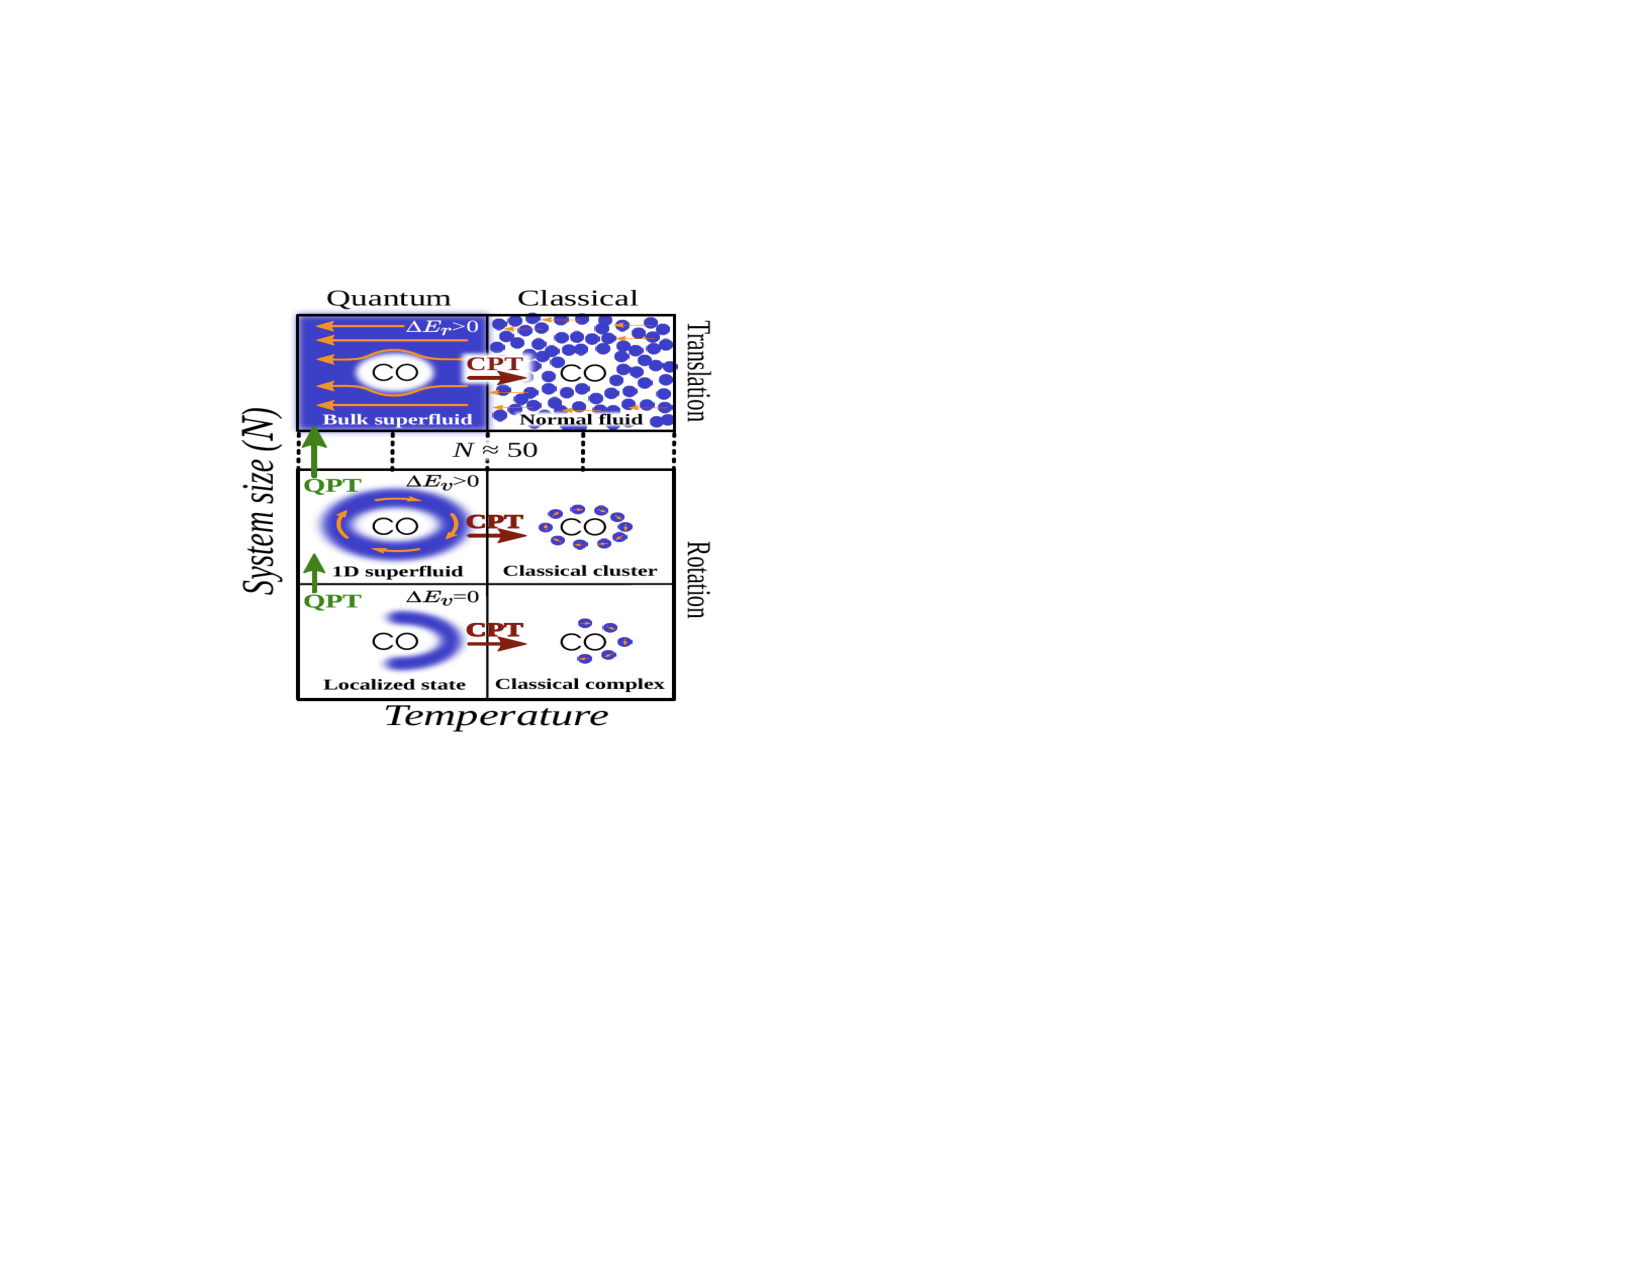
\includegraphics[width=0.8\linewidth]{SysnVTemp}
\captionof{figure}{\color{Green} Figure caption}
\end{center}\vspace{1cm}


%----------------------------------------------------------------------------------------
%	FORTHCOMING
%----------------------------------------------------------------------------------------

\section*{Forthcoming}

\columnbreak


%----------------------------------------------------------------------------------------
%	Empirical Methods
%----------------------------------------------------------------------------------------

\color{Black} % Navy color for the abstract

\section*{Empirical Methods}

Helium is an interesting element with physical properties that are crucial for understanding its behavior when it takes part in chemical reactions.  This element has been known to exist as a gas, liquid and even a solid.  In this experiment, the behavior of linear molecules such OCS (carbonyl sulfide), N2O, CO and HCN is observed by using a plot of rotational constant (B) vs. number of helium atom (N). In this case, small droplets of helium are used as the solvent.   Analyzing the effect of helium on these probe molecules is what helps understand the superfluid behavior of helium.   The temperature at which 4He acts as a superfluid is 0.38K.  When helium atoms are added to one of these molecules, its rotation gets lowered as it starts getting heavier which is expected (see Fig.1).  The strange increase of the rotational constant at N=9 and decrease of moment of inertia becomes evident.  This is considered to be the quantum transition of the reaction in which rotational superfluidity is observed.


%----------------------------------------------------------------------------------------
%	INTRODUCTION - Empirical  %----------------------------------------------------------------------------------------


%----------------------------------------------------------------------------------------
%	RESULTS - MATHEMATICAL
%----------------------------------------------------------------------------------------
\color{Black}
\section*{Results}
In summary, the turnover point in the rotational constants indicate onset of rotational superfluidity.  Rotational superfluidity starts when phase coherence occurs meaning that the molecule becomes completely coated with helium atoms. This cause for this quantum effect has more to do with the geometry of the molecule rather than the intrinsic properties of helium.  It is important to mentions that superfluidity can be described as both rotational and translational superfluidity.  The difference between rotation and translation has to do with the change of location for the molecule even though both refer to motion.  In addition, the molecule moves at a constant velocity and no vortex is formed in translation superfluidity.  Superfluidity for translation occurs at a much higher value of N than for rotation (see Fig. 3).  The alignment of molecules with respect to helium atoms produces rotational wave packets which resemble the behavior of classical rotors.  The rotations observed in this analysis can provide relevant information that can help differentiate quantum rotors from classical ones.

\minipage{0.14\textwidth}
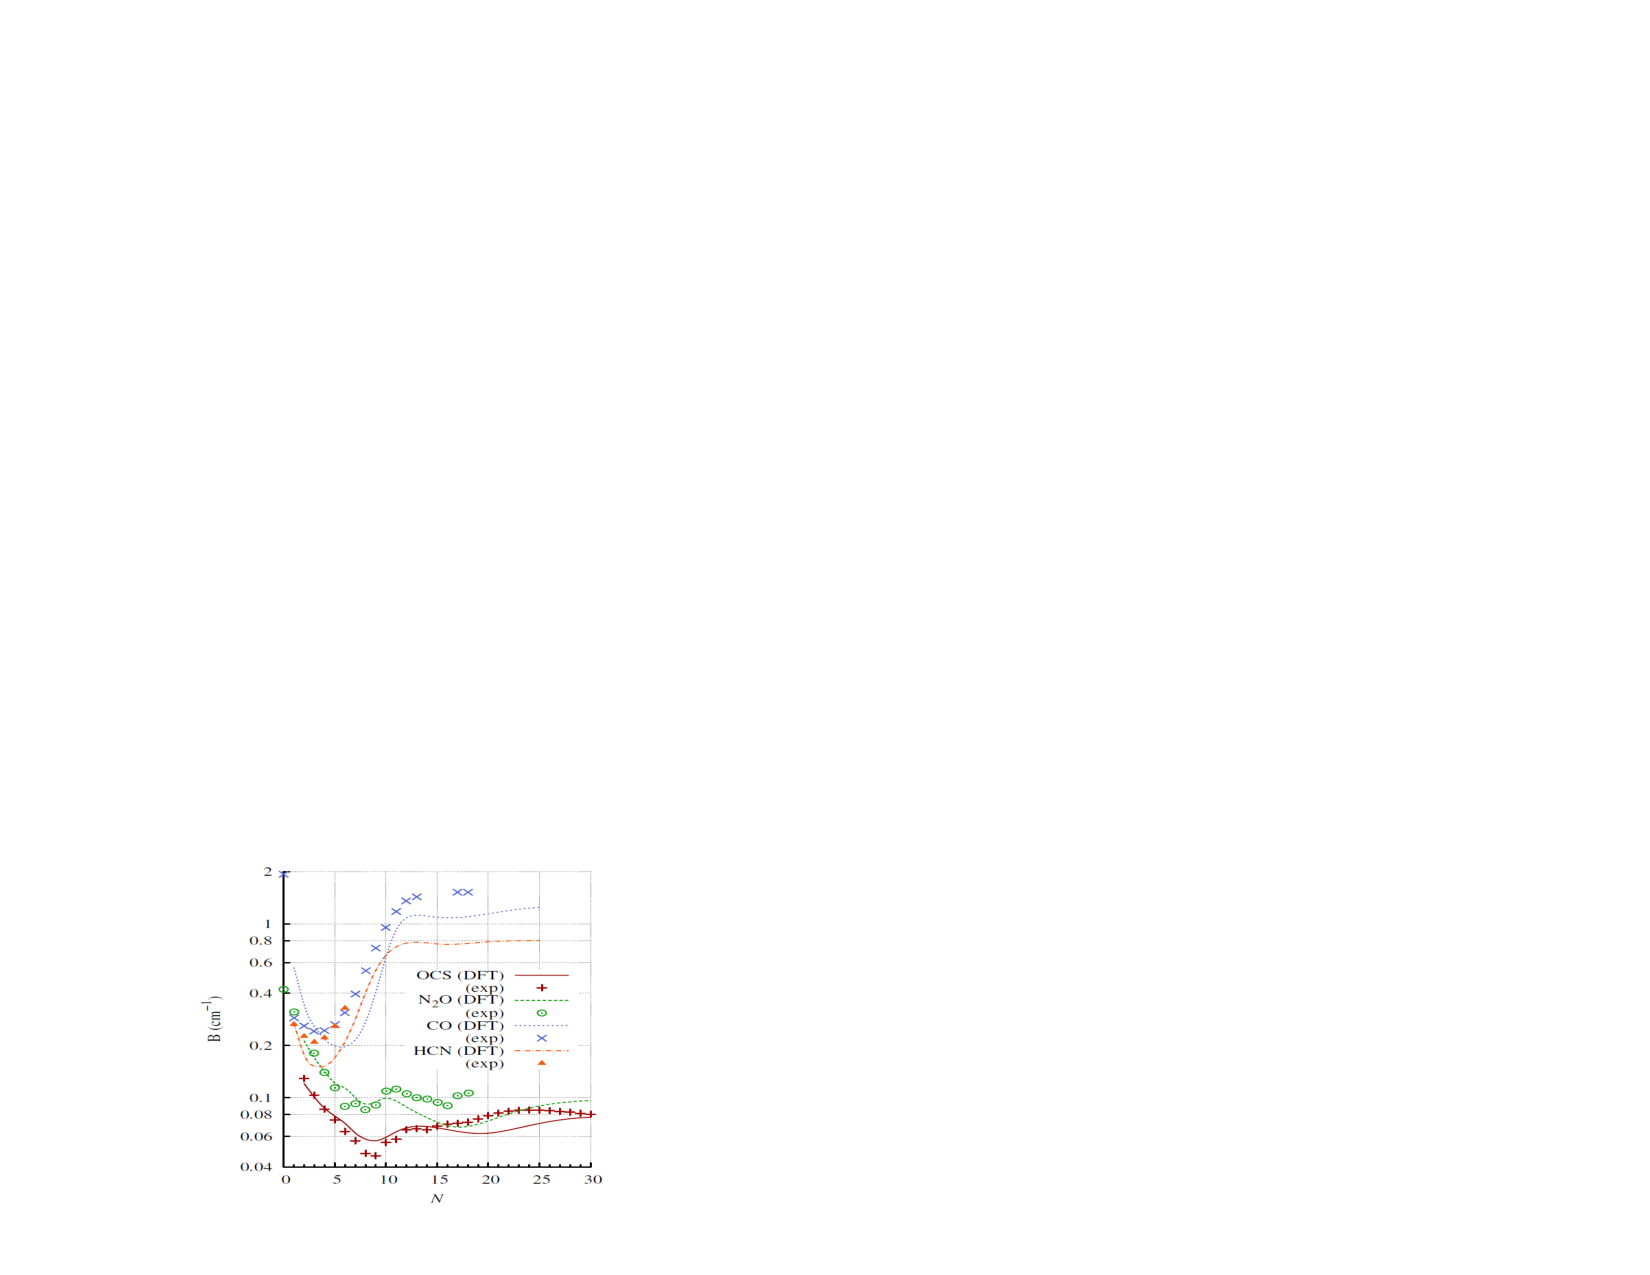
\includegraphics[width=.7\linewidth]{rotConVn}
\captionof{figure}{\color{Navy} Plot of rotational constant ($B$) vs number of helium atoms ($N$) for OCS, N$_2$O and HCN molecules.}
\endminipage\hfill
\minipage{0.14\textwidth}
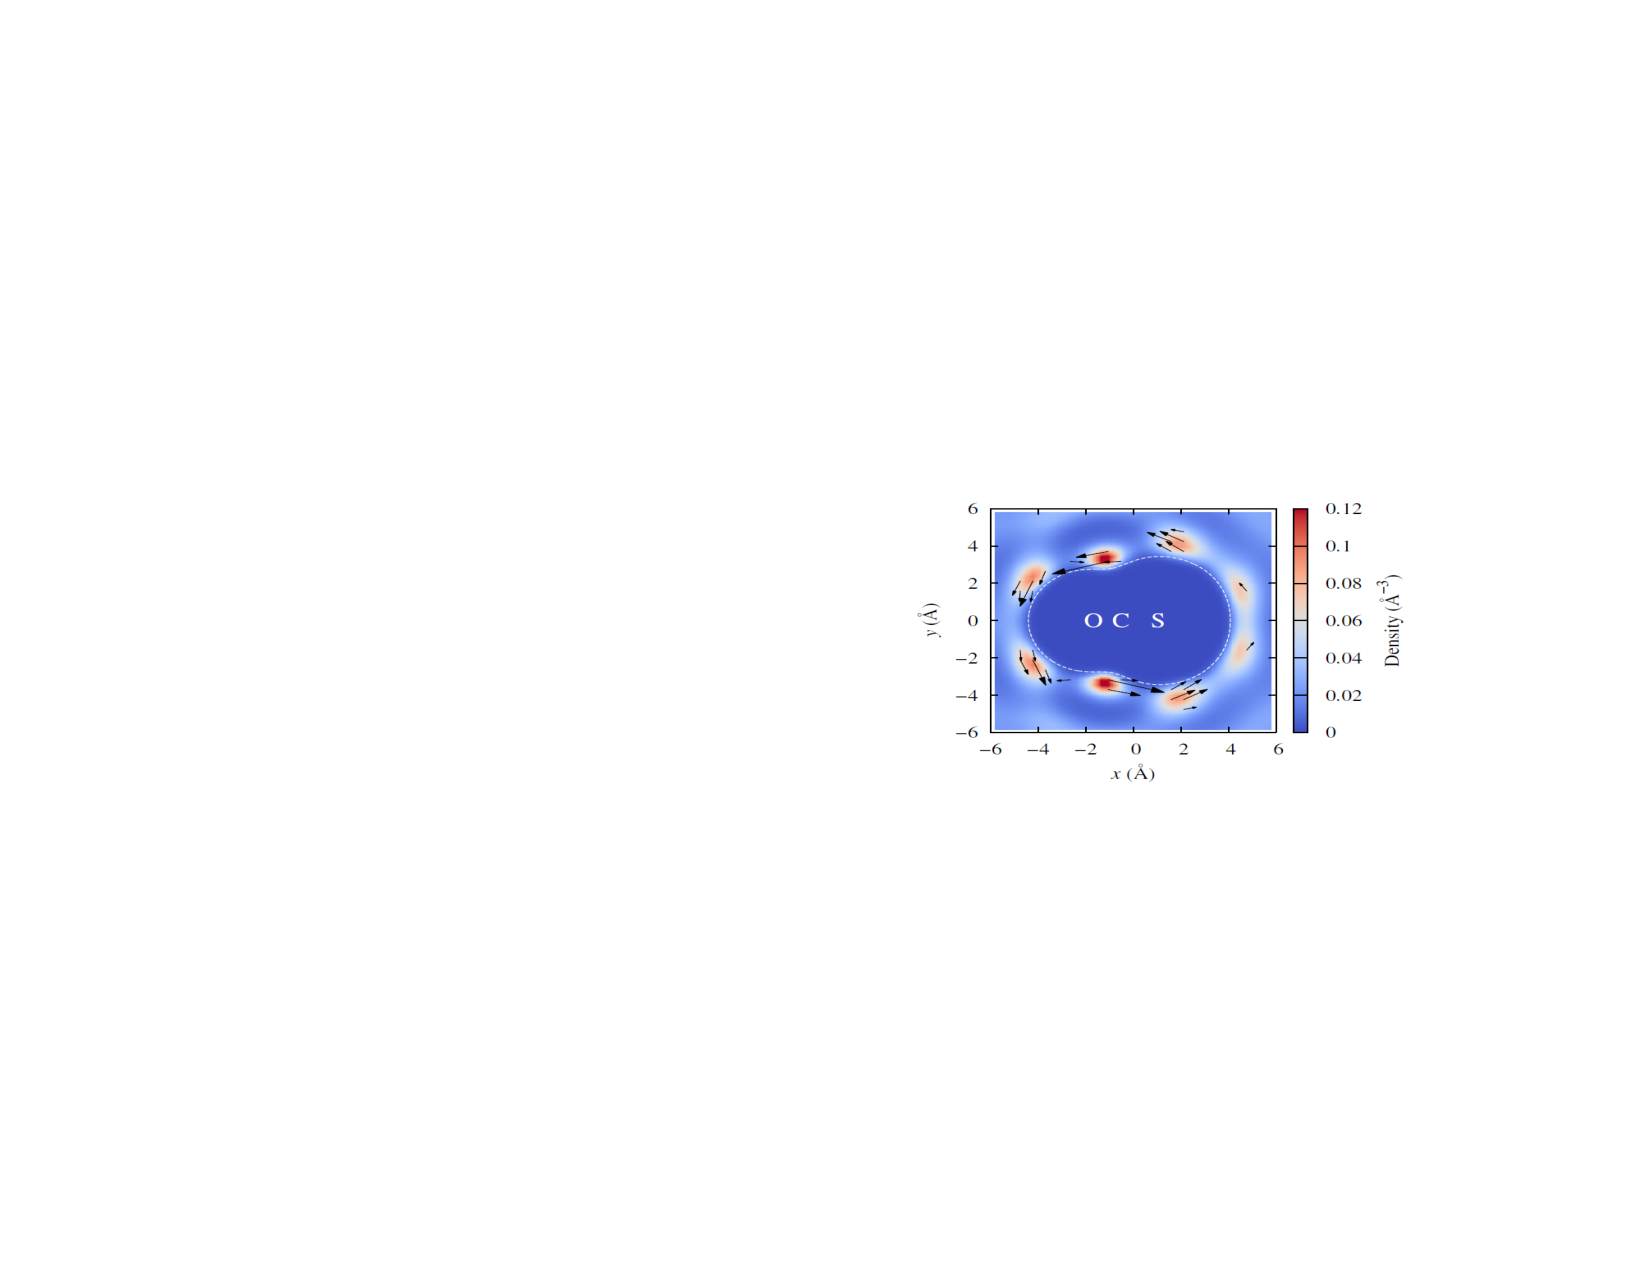
\includegraphics[width=\linewidth]{largeHe}
\captionof{figure}{\color{Navy} Large droplets of helium around OCS which shows a counter-clockwise rotation in 2 dimensions.}
\endminipage



%----------------------------------------------------------------------------------------
%	CONCLUSIONS
%----------------------------------------------------------------------------------------

\section*{Conclusions}
In diam mauris, sagittis ornare est sed, convallis scelerisque eros. Curabitur vel ligula In summary, the turnover point in the rotational constants indicate onset of rotational superfluidity.  Rotational superfluidity starts when phase coherence occurs meaning that the molecule becomes completely coated with helium atoms. This cause for this quantum effect has more to do with the geometry of the molecule rather than the intrinsic properties of helium.  It is important to mentions that superfluidity can be described as both rotational and translational superfluidity.  The difference between rotation and translation has to do with the change of location for the molecule even though both refer to motion.  In addition, the molecule moves at a constant velocity and no vortex is formed in translation superfluidity.  Superfluidity for translation occurs at a much higher value of N than for rotation (see Fig. 3).  The alignment of molecules with respect to helium atoms produces rotational wave packets which resemble the behavior of classical rotors.  The rotations observed in this analysis can provide relevant information that can help differentiate quantum rotors from classical ones.


%----------------------------------------------------------------------------------------
%	REFERENCES
%----------------------------------------------------------------------------------------

\section*{References}
\end{multicols}
\end{document}